\documentclass{beamer}

\usetheme{Warsaw}

\usepackage{verbatim}
\usepackage{xcolor}
\usepackage{listings}
\usepackage{color}
\usepackage[utf8]{inputenc}
\usepackage[T1]{fontenc}
\usepackage{textcomp}
\usepackage{graphicx} 
\usepackage[bulgarian]{babel}
\usepackage{hyperref}
\usepackage{graphicx}

\title{Въведение в Базите данни. Основни понятия и концепции.}
\author{Валентин Гелински}
\institute{ТУ София}
\date{\today} 


\begin{document}
  \begin{frame} 
    \titlepage
  \end{frame}

  \begin{frame}
    \frametitle{За курса}
    \begin{itemize}
      \item{Оценяване}
      \item{Курсови задачи}
    \end{itemize}
  \end{frame}

  \begin{frame}
    \frametitle{Въведение в базите данни}
    \framesubtitle{Или защо си усложняваме живота}
    \begin{itemize}
      \item{Оптимизация по обем (памет)}
      \item{Оптимизация по скорост}
      \item{Консистентност на данните}
      \item{Независимост от кода на програмата}
      \item{Сигурност}
    \end{itemize}
  \end{frame}

  \begin{frame}
    \frametitle{СУБД}
    \framesubtitle{Database Managment System}
    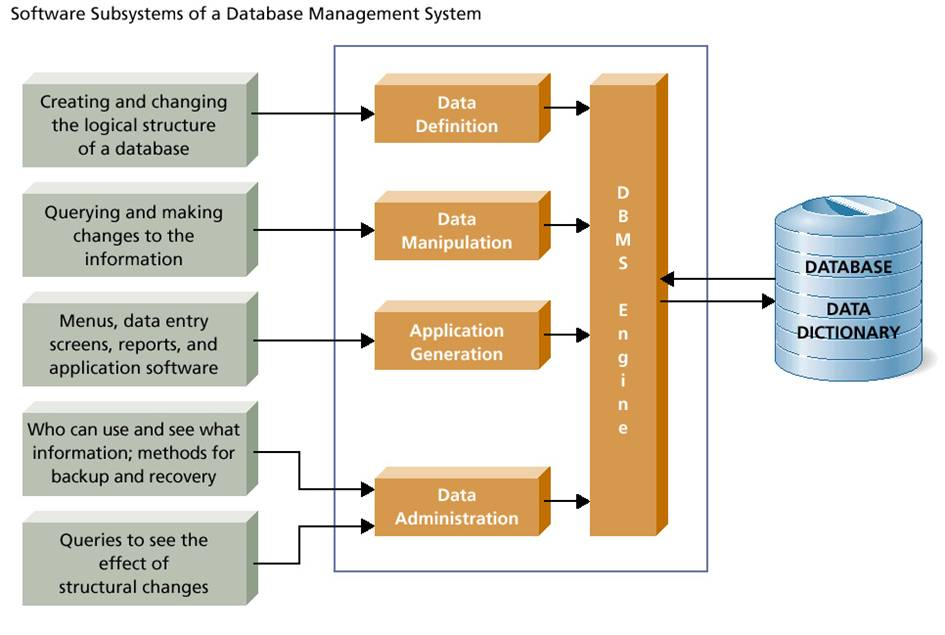
\includegraphics[width=250px]{img/rdbms}
  \end{frame}

  \begin{frame}
    \frametitle{ER model}
    \begin{itemize}
      \item{Обект}
      \item{Класове обекти}
      \item{Атрибути}
      \item{Връзки}
      \begin{itemize}
        \item{Връзки 1:1}
        \item{Връзки 1:М}
        \item{Връзки М:М}
      \end{itemize}
      \item{Характеризиращи обекти}
      \item{Подклас обекти}
    \end{itemize}
  \end{frame}

  \begin{frame}
    \frametitle{Обект}
    
\includegraphics[width=250px]{img/doge}
  \end{frame}

  \begin{frame}
    \frametitle{Клас обекти}
    \framesubtitle{Entity}
    \begin{block}{Клас обекти}
      Множество от обекти, които имат сходни и общи свойства.
    \end{block}
    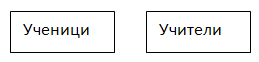
\includegraphics[width=250px]{img/entity}
  \end{frame}

  \begin{frame}
    \frametitle{Атрибут}
    \framesubtitle{Atribute}
    \begin{block}{Атрибут}
       Свойство на даден обект в даден клас
    \end{block}
    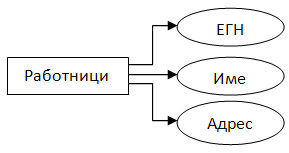
\includegraphics[width=250px]{img/atribute}
  \end{frame}

  \begin{frame}
    \frametitle{Линк}
    \framesubtitle{Relatioship}
    \begin{block}{Линк}
      Показва връзката между класовете в структурата на базата.
    \end{block}
    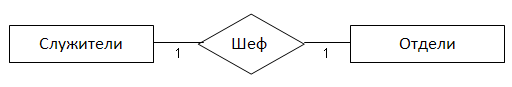
\includegraphics[width=250px]{img/relation_11}\\
    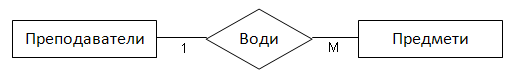
\includegraphics[width=250px]{img/relation_1m}\\
    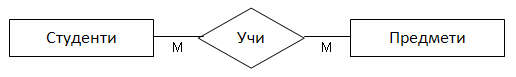
\includegraphics[width=250px]{img/relation_mm}
  \end{frame}
  
  \begin{frame}
    \frametitle{Характеризиращ обект}
    \framesubtitle{Weak entity}
    \begin{block}{Характеризиращ обект}
       Обект от предметната област, чието съществуване е невъзможно самостоятелно.
    \end{block}
    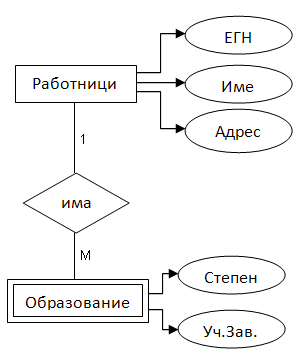
\includegraphics[width=100px]{img/weak_entity}
  \end{frame}

  \begin{frame}
    \frametitle{Подклас обекти}
    \framesubtitle{Subclass}
    \begin{block}{Подклас обекти}
      Обекти, които притежават всички свойства на даден базов клас обекти, но имат допълнителни свои атрибути.
    \end{block}
    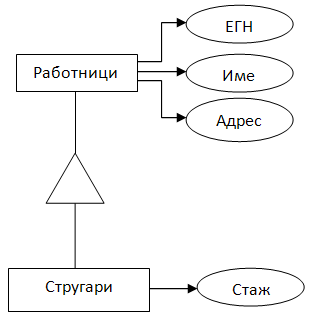
\includegraphics[width=100px]{img/subclass}
  \end{frame}
  
  
\end{document}

